% Chapter Template

\chapter{Requisits} % Main chapter title

\label{Requisits} % Change X to a consecutive number; for referencing this chapter elsewhere, use \ref{ChapterX}

\section{Propietats i hipòtesis sobre el domini}

Per a poder desenvolupar aquest projecte, s’ha considerat necessari definir una sèrie d’expectatives sobre l’ús del sistema.
\begin{itemize}
\item{}\textbf{Connexió a internet}\\
L’usuari té connexió a internet en tot moment ja que es necessita a l’hora
de guardar i consultar dades, i a l’hora d’accedir a serveis web.
\item{}\textbf{Ús del sistema}\\
Els usuaris utilitzaran el sistema d’acord amb la finalitat per al qual ha
sigut creat sense fer-ne un mal us o emprenen accions malicioses que puguin trencar la integritat del sistema. Tot i així, s’implementaran mitjants de seguretat per protegir l’aplicació en aquest aspecte.
\item{}\textbf{Obtenció de dades correctes}\\
 Les dades que s’obtenen de serveis web són
correctes i actualitzades.

\end{itemize}

\section{Restriccions}
\begin{itemize}
\item[]\textbf{Restricció de la solució}
\begin{itemize}
\item{}Descripció: L’aplicació serà desenvolupada com a aplicació mòbil Android.
\item{}Justificació: Els dispositius mòbils estan sempre aprop de l’usuari i
disponibles per al seu ús, a més, en els últims anys s’ha extés l’ús
d’internet al mòbil. Pel que fa al sistema operatiu, degut a la limitació temporal del treball i a que té una quota de mercat molt gran a
Espanya s’ha optat per la implementació en Android, encara que no
es descarten altres sistemes operatius en un futur.
\end{itemize}
\item[]\textbf{Restricció temporal}
\begin{itemize}
\item{}Descripció: El sistema ha d’estar acabat a meitats de juny de 2017.
\item{}Justificació: S’estableix una data límit per presentar el projecte.
\end{itemize}
\item[]\textbf{Restricció econòmica}
\begin{itemize}
\item{}Descripció: El desenvolupament del projecte es durà a terme sense
cap cost econòmic.
\item{}Justificació: Com que no es disposa de cap inversió econòmica i el
projecte es desenvolupa en un entorn acadèmic les eines i serveis uti-
litzats suposaran un cost molt baix.
\end{itemize}
\end{itemize}

\section{Diagrama de casos d'ús}
En la figura 5.1 es mostra el diagrama de casos d’ús del sistema sense tenir en compte la gestió d'usuaris.

\begin{figure}[!h]
\centering
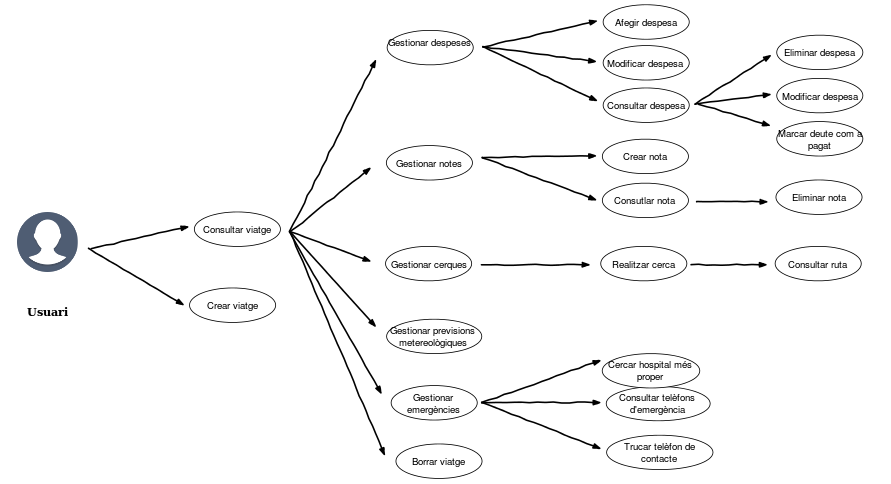
\includegraphics[scale=0.65]{Figures/casosUs.png}
\caption{Diagrama de casos d'ús}
\end{figure}

\section{Casos dús}

\newcolumntype{L}{>{\centering}m{0.75cm}}
\newcolumntype{M}{m{9cm}}
\newcolumntype{T}{m{12cm}}

\newcommand\tab[1][0.75cm]{\hspace*{#1}}

\newcolumntype{L}{>{\centering}m{0.75cm}}
\newcolumntype{M}{m{9cm}}
\newcolumntype{T}{m{12cm}}

\newcommand\tab[1][0.75cm]{\hspace*{#1}}

\begin{table}[!h]
\begin{tabular}{|l|L|l|}
\hline
\textbf{Cas d'ús }& \#1 &  Registrar-se al sistema  \\ \hline
\textbf{Actor principal} & \multicolumn{ 2}{l|}{Usuari} \\ \hline
\textbf{Precondició} & \multicolumn{ 2}{M|}{L'usuari té l'aplicació instal·lada al seu dispositiu.} \\ \hline
\textbf{Trigger} & \multicolumn{ 2}{M|}{L'usuari es vol registrar al sistema.} \\ \hline
\multicolumn{ 3}{|T|}{\textbf{Escenari principal d’èxit}} \\ \hline
\multicolumn{ 3}{|T|}{1. L’usuari selecciona el botó de registrar-se utilitzant el seu compte de Google.}\\
\multicolumn{ 3}{|T|}{2. El sistema redirigeix el nou registre a Google.
}\\
\multicolumn{ 3}{|T|}{3. L’usuari introdueix el seu correu electrònic i la seva contrassenya.
}\\
\multicolumn{ 3}{|T|}{4. Google valida les dades.
}\\
\multicolumn{ 3}{|T|}{5. L’usuari accepta donar permisos a l’aplicació per obtenir les dades del seu perfil.}\\
\multicolumn{ 3}{|T|}{6. El sistema registra l’usuari i inicia sessió automàticament.}\\
\hline
\multicolumn{ 3}{|T|}{\textbf{Extensions}} \\ \hline
\multicolumn{ 3}{|T|}{4.a El sistema detecta algun error en els camps introduïts.
} \\
\multicolumn{ 3}{|T|}{\tab4.a.1 El sistema notifica a l’usuari de l’error.
} \\
\multicolumn{ 3}{|T|}{\tab4.a.2 Es torna al pas 3.
} \\
\multicolumn{ 3}{|T|}{5.a L’usuari no dona permisos a l’aplicació per obtenir les dades del seu perfil.} \\
\multicolumn{ 3}{|T|}{\tab5.a.1 El sistema torna al pas 1.
} \\\hline
\end{tabular}
\label{}
\caption{Cas d'ús \textit{Registrar-se al sistema}}
\end{table}

\begin{table}[!h]
\begin{tabular}{|l|L|l|}
\hline
\textbf{Cas d'ús }& \#2 &  Iniciar sessió al sistema  \\ \hline
\textbf{Actor principal} & \multicolumn{ 2}{l|}{Usuari} \\ \hline
\textbf{Precondició} & \multicolumn{ 2}{M|}{L’usuari està registrat al sistema.} \\ \hline
\textbf{Trigger} & \multicolumn{ 2}{M|}{L’usuari vol iniciar sessió al sistema.} \\ \hline
\multicolumn{ 3}{|T|}{\textbf{Escenari principal d’èxit}} \\ \hline
\multicolumn{ 3}{|T|}{1. L’usuari introdueix el seu correu electrònic i contrasenya, i indica al sistema que vol identificar-se.}\\
\multicolumn{ 3}{|T|}{2. El sistema valida les dades, identifica l’usuari i redirigeix a l’usuari a la pantalla de viatge actual.
}\\
\hline
\multicolumn{ 3}{|T|}{\textbf{Extensions}} \\ \hline
\multicolumn{ 3}{|T|}{2.a El sistema detecta algun error en els camps introduïts.
} \\
\multicolumn{ 3}{|T|}{\tab2.a.1 El sistema notifica a l’usuari que hi ha dades incorrectes.
} \\
\multicolumn{ 3}{|T|}{\tab2.a.2 Es torna al pas 1.
} \\
\multicolumn{ 3}{|T|}{3.a L’usuari no té cap viatge actiu.
} \\
\multicolumn{ 3}{|T|}{\tab3.a.1 El sistema redirigeix l’usuari a la pantalla de llista de viatges realitzats.
} \\\hline
\end{tabular}
\label{}
\caption{Cas d'ús \textit{Iniciar sessió al sistema}}
\end{table}

\begin{table}[!h]
\begin{tabular}{|l|L|l|}
\hline
\textbf{Cas d'ús }& \#3 & Tancar sessió al sistema   \\ \hline
\textbf{Actor principal} & \multicolumn{ 2}{l|}{Usuari} \\ \hline
\textbf{Precondició} & \multicolumn{ 2}{M|}{L’usuari ha iniciat sessió al sistema.} \\ \hline
\textbf{Trigger} & \multicolumn{ 2}{M|}{L’usuari vol tancar la sessió al sistema.} \\ \hline
\multicolumn{ 3}{|T|}{\textbf{Escenari principal d’èxit}} \\ \hline
\multicolumn{ 3}{|T|}{1. L’usuari indica al sistema que vol tancar sessió.
}\\
\multicolumn{ 3}{|T|}{2. El sistema es desvincula de les dades de l’usuari actual i redirigeix l’aplicació a la pantalla d’iniciar sessió.}\\\hline
\end{tabular}
\label{}
\caption{Cas d'ús \textit{Tancar sessió al sistema}}
\end{table}

\clearpage

\begin{table}[!h]
\begin{tabular}{|l|L|l|}
\hline
\textbf{Cas d'ús }& \#4 & Crear viatge  \\ \hline
\textbf{Actor principal} & \multicolumn{ 2}{l|}{Usuari} \\ \hline
\textbf{Precondició} & \multicolumn{ 2}{M|}{L’usuari ha iniciat sessió al sistema.} \\ \hline
\textbf{Trigger} & \multicolumn{ 2}{M|}{L’usuari vol iniciar un nou viatge.} \\ \hline
\multicolumn{ 3}{|T|}{\textbf{Escenari principal d’èxit}} \\ \hline
\multicolumn{ 3}{|T|}{1. L’usuari indica que vol iniciar un nou viatge.
}\\
\multicolumn{ 3}{|T|}{2. El sistema redirecciona l’usuari a la pàgina de creació de viatge.
}\\
\multicolumn{ 3}{|T|}{3. L’usuari introdueix el nom del viatge,el destí, la data d’inici i la data final, el nom i correu electrònic de tots els viatgers que formaran part del viatge i indica que vol iniciar el viatge.
}\\
\multicolumn{ 3}{|T|}{4. El sistema valida les dades i presenta a l’usuari el formulari de preferències.
}\\
\multicolumn{ 3}{|T|}{5. L’usuari respon el formulari i indica que ja ha acabat.}\\
\multicolumn{ 3}{|T|}{6. El sistema guarda el resultat del formulari i presenta a l'usuari el formulari per a que introdueixi les dades del contacte d'emergència.}\\
\multicolumn{ 3}{|T|}{7. L'usuari introdueix les dades i indica que ja ha acabat.}\\
\multicolumn{ 3}{|T|}{8. El sistema guarda el resultat, crea el viatge amb les dades introduïdes i redirigeix l'usuari a la pantalla principal del viatge.}\\
\hline
\multicolumn{ 3}{|T|}{\textbf{Extensions}} \\ \hline
\multicolumn{ 3}{|T|}{4.a El sistema detecta errors en les dades introduïdes.
} \\
\multicolumn{ 3}{|T|}{\tab4.a.1 El sistema notifica a l’usuari que hi ha dades incorrectes.} \\
\multicolumn{ 3}{|T|}{\tab4.a.2 Es torna al pas 2.} \\
\multicolumn{ 3}{|T|}{6.a El sistema detecta que no s’ha completat el formulari.
} \\
\multicolumn{ 3}{|T|}{\tab6.a.1 El sistema notifica a l’usuari que hi ha camps incomplets.} \\
\multicolumn{ 3}{|T|}{\tab6.a.2 Es torna al pas 5.} \\\hline
\end{tabular}
\label{}
\caption{Cas d'ús \textit{Crear viatge}}
\end{table}

\begin{table}[!h]
\begin{tabular}{|l|L|l|}
\hline
\textbf{Cas d'ús }& \#5 &  Consultar llista de viatges \\ \hline
\textbf{Actor principal} & \multicolumn{ 2}{l|}{Usuari} \\ \hline
\textbf{Precondició} & \multicolumn{ 2}{M|}{L’usuari ha iniciat sessió al sistema.} \\ \hline
\textbf{Trigger} & \multicolumn{ 2}{M|}{L’usuari vol consultar viatges o ha iniciat sessió i no té cap viatge en curs.} \\ \hline
\multicolumn{ 3}{|T|}{\textbf{Escenari principal d’èxit}} \\ \hline
\multicolumn{ 3}{|T|}{1. L’usuari indica que vol consultar els seus viatges.}\\
\multicolumn{ 3}{|T|}{2. El sistema redirigeix l’usuari a la pantalla de llista de viatges.}\\\hline
\end{tabular}
\label{}
\caption{Cas d'ús \textit{Consultar llista de viatges}}
\end{table}

\clearpage

\begin{table}[!h]
\begin{tabular}{|l|L|l|}
\hline
\textbf{Cas d'ús }& \#6 & Consultar despeses   \\ \hline
\textbf{Actor principal} & \multicolumn{ 2}{l|}{Usuari} \\ \hline
\textbf{Precondició} & \multicolumn{ 2}{M|}{L’usuari ha accedit a un viatge i ha iniciat sessió.} \\ \hline
\textbf{Trigger} & \multicolumn{ 2}{M|}{L’usuari vol accedir a la funcionalitat gestió de despeses.} \\ \hline
\multicolumn{ 3}{|T|}{\textbf{Escenari principal d’èxit}} \\ \hline
\multicolumn{ 3}{|T|}{1. L’usuari indica que vol accedir a la funcionalitat gestió de despeses.}\\
\multicolumn{ 3}{|T|}{2. El sistema el redirigeix a la pantalla d’estadístiques de despeses on es mostra la despesa total, la mitjana \euro/dia i la llista de les despeses.}\\
\hline
\end{tabular}
\label{}
\caption{Cas d'ús \textit{Consultar despeses}}
\end{table}


\begin{table}[!h]
\begin{tabular}{|l|L|l|}
\hline
\textbf{Cas d'ús }& \#7 & Afegir nova despesa  \\ \hline
\textbf{Actor principal} & \multicolumn{ 2}{l|}{Usuari} \\ \hline
\textbf{Precondició} & \multicolumn{ 2}{M|}{L’usuari ha accedit a la funcionaltiat gestió de despeses compartides.} \\ \hline
\textbf{Trigger} & \multicolumn{ 2}{M|}{L’usuari vol afegir una nova despesa.} \\ \hline
\multicolumn{ 3}{|T|}{\textbf{Escenari principal d’èxit}} \\ \hline
\multicolumn{ 3}{|T|}{1. L’usuari indica que vol afegir una nova despesa.}\\
\multicolumn{ 3}{|T|}{2. El sistema redirigeix l’usuari a la pantalla de nova despesa.}\\
\multicolumn{ 3}{|T|}{3. L’usuari introdueix la quantitat que paga.}\\
\multicolumn{ 3}{|T|}{4. El sistema guarda les dades, crea la nova despesa, actualitza les estadístiques.}\\
\hline
\multicolumn{ 3}{|T|}{\textbf{Extensions}} \\ \hline
\multicolumn{ 3}{|T|}{3.a L’usuari notifica que vol crear un deute.} \\
\multicolumn{ 3}{|T|}{\tab3.a.1  L’usuari indica el participant deutor i la quantitat.
} \\
\multicolumn{ 3}{|T|}{\tab3.a.2  El sistema guarda els deutes i envia un avís als deutors.} \\
\multicolumn{ 3}{|T|}{4.a El sistema detecta dades incompatibles introduïdes per l’usuari.} \\
\multicolumn{ 3}{|T|}{\tab4.a.1 El sistema notifica a l’usuari que s’han detectat dades incompatibles.} \\
\multicolumn{ 3}{|T|}{\tab4.a.2 Es torna al pas 2.} \\\hline
\end{tabular}
\label{}
\caption{Cas d'ús \textit{Afegir nova despesa}}
\end{table}

\clearpage

\begin{table}[!h]
\begin{tabular}{|l|L|l|}
\hline
\textbf{Cas d'ús }& \#8 & Eliminar despesa   \\ \hline
\textbf{Actor principal} & \multicolumn{ 2}{l|}{Usuari} \\ \hline
\textbf{Precondició} & \multicolumn{ 2}{M|}{L’usuari ha accedit a la funcionalitat gestió de despeses compartides i ha creat almenys una despesa.} \\ \hline
\textbf{Trigger} & \multicolumn{ 2}{M|}{L’usuari vol eliminar una despesa.} \\ \hline
\multicolumn{ 3}{|T|}{\textbf{Escenari principal d’èxit}} \\ \hline
\multicolumn{ 3}{|T|}{1. L’usuari indica que vol eliminar una despesa en concret.
}\\
\multicolumn{ 3}{|T|}{2. El sistema mostra un diàleg on pregunta si està segur de voler eliminar la despesa.}\\
\multicolumn{ 3}{|T|}{3. L’usuari confirma que vol eliminar la despesa.}\\
\multicolumn{ 3}{|T|}{4. El sistema elimina la despesa, elimina els deutes relacionats i actualitza les estadístiques de despeses.}\\
\hline
\multicolumn{ 3}{|T|}{\textbf{Extensions}} \\ \hline
\multicolumn{ 3}{|T|}{3.a L’usuari cancel·la l’eliminació de la despesa.} \\
\multicolumn{ 3}{|T|}{\tab3.a.1 Es torna a la pantalla de gestió de despeses compartides.} \\ \hline
\end{tabular}
\label{}
\caption{Cas d'ús \textit{Eliminar despesa}}
\end{table}
\begin{table}[!h]
\begin{tabular}{|l|L|l|}
\hline
\textbf{Cas d'ús }& \#9 &  Consultar deutes de despesa \\ \hline
\textbf{Actor principal} & \multicolumn{ 2}{l|}{Usuari} \\ \hline
\textbf{Precondició} & \multicolumn{ 2}{M|}{L’usuari ha accedit a la funcionalitat de gestió de despeses.} \\ \hline
\textbf{Trigger} & \multicolumn{ 2}{M|}{ L’usuari vol consultar els deutes d’una despesa.} \\ \hline
\multicolumn{ 3}{|T|}{\textbf{Escenari principal d’èxit}} \\ \hline
\multicolumn{ 3}{|T|}{1. L’usuari indica que vol consultar els deutes d’una despesa.}\\
\multicolumn{ 3}{|T|}{2. El sistema redirigeix l’usuari a la pantalla de consulta de deutes d’una despesa on mostra la llista dels deutes de la despesa indicada.}\\\hline
\end{tabular}
\label{}
\caption{Cas d'ús \textit{Consultar deutes de despesa}}
\end{table}
\begin{table}[!h]
\begin{tabular}{|l|L|l|}
\hline
\textbf{Cas d'ús }& \#10 & Cobrar deute   \\ \hline
\textbf{Actor principal} & \multicolumn{ 2}{l|}{Usuari} \\ \hline
\textbf{Precondició} & \multicolumn{ 2}{M|}{L’usuari ha accedit a la consulta de deutes d’una despesa i almenys existeix un deute per aquella despesa.} \\ \hline
\textbf{Trigger} & \multicolumn{ 2}{M|}{L’usuari vol marcar com a cobrat un deute.} \\ \hline
\multicolumn{ 3}{|T|}{\textbf{Escenari principal d’èxit}} \\ \hline
\multicolumn{ 3}{|T|}{1. L’usuari indica que vol marcar com a cobrat un deute.}\\
\multicolumn{ 3}{|T|}{2. El sistema mostra un diàleg on pregunta si està segur de voler marcar com a cobrat el deute.}\\
\multicolumn{ 3}{|T|}{3. L’usuari confirma que vol marcar com a cobrat el deute.}\\
\multicolumn{ 3}{|T|}{4. El sistema marca que el deute està cobrat.}\\
\hline
\multicolumn{ 3}{|T|}{\textbf{Extensions}} \\ \hline
\multicolumn{ 3}{|T|}{3.a L’usuari cancel·la el cobrament del deute.} \\
\multicolumn{ 3}{|T|}{\tab3.a.1 Es torna a la pantalla de consultar deutes d’una despesa.} \\\hline
\end{tabular}
\label{}
\caption{Cas d'ús \textit{Cobrar deute}}
\end{table}
\begin{table}[!h]
\begin{tabular}{|l|L|l|}
\hline
\textbf{Cas d'ús }& \#11 & Modificar despesa   \\ \hline
\textbf{Actor principal} & \multicolumn{ 2}{l|}{Usuari} \\ \hline
\textbf{Precondició} & \multicolumn{ 2}{M|}{L’usuari ha accedit a la consulta de despeses i té almenys una despesa.} \\ \hline
\textbf{Trigger} & \multicolumn{ 2}{M|}{L’usuari vol modificar una despesa.} \\ \hline
\multicolumn{ 3}{|T|}{\textbf{Escenari principal d’èxit}} \\ \hline
\multicolumn{ 3}{|T|}{1. L’usuari indica que vol modificar una despesa.}\\
\multicolumn{ 3}{|T|}{2. El sistema redirigeix l’usuari a la pantalla de modificació de despesa.}\\
\multicolumn{ 3}{|T|}{3. L’usuari introdueix els canvis desitjats i indica que ja ha acabat.}\\
\multicolumn{ 3}{|T|}{4. El sistema guarda els canvis i redirigeix l’usuari a la pantalla de consulta de despeses.}\\
\hline
\multicolumn{ 3}{|T|}{\textbf{Extensions}} \\ \hline
\multicolumn{ 3}{|T|}{3.a L’usuari cancel·la la modificació de la despesa.} \\
\multicolumn{ 3}{|T|}{\tab3.a.1 Es torna a la pantalla de consultar deutes d’una despesa.} \\\hline
\end{tabular}
\label{}
\caption{Cas d'ús \textit{Modificar despesa}}
\end{table}

\begin{table}[!h]
\begin{tabular}{|l|L|l|}
\hline
\textbf{Cas d'ús }& \#12 & Gestionar cerques   \\ \hline
\textbf{Actor principal} & \multicolumn{ 2}{l|}{Usuari} \\ \hline
\textbf{Precondició} & \multicolumn{ 2}{M|}{L’usuari ha iniciat sessió i té un viatge en curs.} \\ \hline
\textbf{Trigger} & \multicolumn{ 2}{M|}{L’usuari vol accedir a la funcionalitat de cerques.} \\ \hline
\multicolumn{ 3}{|T|}{\textbf{Escenari principal d’èxit}} \\ \hline
\multicolumn{ 3}{|T|}{1. L’usuari indica que vol accedir a la funcionalitat de cerques.}\\
\multicolumn{ 3}{|T|}{2. El sistema redirigeix l’usuari a la pantalla de realitzar una cerca.}\\\hline
\end{tabular}
\label{}
\caption{Cas d'ús \textit{Gestionar cerques}}
\end{table}

\begin{table}[!h]
\begin{tabular}{|l|L|l|}
\hline
\textbf{Cas d'ús }& \#13 & Realitzar una cerca   \\ \hline
\textbf{Actor principal} & \multicolumn{ 2}{l|}{Usuari} \\ \hline
\textbf{Precondició} & \multicolumn{ 2}{M|}{L’usuari ha accedit a la funcionalitat de gestionar cerques.} \\ \hline
\textbf{Trigger} & \multicolumn{ 2}{M|}{L’usuari vol realitzar una cerca.} \\ \hline
\multicolumn{ 3}{|T|}{\textbf{Escenari principal d’èxit}} \\ \hline
\multicolumn{ 3}{|T|}{1. L’usuari indica què vol cercar i la seva localització.}\\
\multicolumn{ 3}{|T|}{2. El sistema crida a la API de cerques amb els paràmetres que ha introduït l’usuari.}\\
\multicolumn{ 3}{|T|}{3. El sistema mostra els resultats que retorna la API ordenats tenint en compte l’estil de viatjar de l’usuari.}\\
\hline
\multicolumn{ 3}{|T|}{\textbf{Extensions}} \\ \hline
\multicolumn{ 3}{|T|}{1.a El sistema detecta que l’usuari no té activat el GPS al seu dispositiu.} \\
\multicolumn{ 3}{|T|}{\tab1.a.1 El sistema demana si pot activar el GPS.} \\
\multicolumn{ 3}{|T|}{\tab1.a.2 L’usuari accepta activar el GPS.} \\
\multicolumn{ 3}{|T|}{\tab1.a.3 El sistema executa el pas 2.} \\
\multicolumn{ 3}{|T|}{\tab1.a.2.a L’usuari no accepta activar el GPS.} \\
\multicolumn{ 3}{|T|}{\tab\tab1.a.2.a.1 El sistema retorna a la pantalla inicial del cas d’ús.} \\
\multicolumn{ 3}{|T|}{2.a El sistema no pot comunicar-se amb la API per falta de connexió a internet.} \\
\multicolumn{ 3}{|T|}{\tab2.a.1 El sistema notifica a l’usuari.} \\\hline
\end{tabular}
\label{}
\caption{Cas d'ús \textit{Realitzar una cerca}}
\end{table}

\begin{table}[!h]
\begin{tabular}{|l|L|l|}
\hline
\textbf{Cas d'ús }& \#14 & Consultar ruta   \\ \hline
\textbf{Actor principal} & \multicolumn{ 2}{l|}{Usuari} \\ \hline
\textbf{Precondició} & \multicolumn{ 2}{M|}{L’usuari ha realitzat una cerca.} \\ \hline
\textbf{Trigger} & \multicolumn{ 2}{M|}{L’usuari vol consultar com arribar fins a un dels punts de la cerca.} \\ \hline
\multicolumn{ 3}{|T|}{\textbf{Escenari principal d’èxit}} \\ \hline
\multicolumn{ 3}{|T|}{1. L’usuari indica a quin resultat de cerca vol arribar}\\
\multicolumn{ 3}{|T|}{2. El sistema fa una crida a la API i redirigeix l’usuari a la pantalla de ruta on mostra el resultat obtingut representat al mapa.}\\
\hline
\multicolumn{ 3}{|T|}{\textbf{Extensions}} \\ \hline
\multicolumn{ 3}{|T|}{1.a El sistema detecta que l’usuari no té activat el GPS al seu dispositiu.} \\
\multicolumn{ 3}{|T|}{\tab1.a.1 El sistema demana si pot activar el GPS.} \\
\multicolumn{ 3}{|T|}{\tab1.a.2 L’usuari accepta activar el GPS.} \\
\multicolumn{ 3}{|T|}{\tab1.a.3 El sistema executa el pas 2.} \\
\multicolumn{ 3}{|T|}{\tab1.a.2.a L’usuari no accepta activar el GPS.} \\
\multicolumn{ 3}{|T|}{\tab\tab1.a.2.a.1 El sistema retorna a la pantalla inicial del cas d’ús.} \\
\multicolumn{ 3}{|T|}{2.a El sistema no pot comunicar-se amb la API per falta de connexió a internet.} \\
\multicolumn{ 3}{|T|}{\tab2.a.1 El sistema notifica a l’usuari.} \\\hline
\end{tabular}
\label{}
\caption{Cas d'ús \textit{Consultar ruta}}
\end{table}

\begin{table}[!h]
\begin{tabular}{|l|L|l|}
\hline
\textbf{Cas d'ús }& \#15 & Consultar previsió metereològica  \\ \hline
\textbf{Actor principal} & \multicolumn{ 2}{l|}{Usuari} \\ \hline
\textbf{Precondició} & \multicolumn{ 2}{M|}{L'usuari té un viatge en curs i ha iniciat sessió.} \\ \hline
\textbf{Trigger} & \multicolumn{ 2}{M|}{L'usuari vol accedir a la funcionalitat de consultar previsió metereològica.} \\ \hline
\multicolumn{ 3}{|T|}{\textbf{Escenari principal d’èxit}} \\ \hline
\multicolumn{ 3}{|T|}{1. L'usuari indica que vol accedir a la funcionalitat de consultar previsió metereològica.}\\
\multicolumn{ 3}{|T|}{2. El sistema redirigeix l'usuari a la pantalla de previsió metereològica.}\\\hline
\end{tabular}
\label{}
\caption{Cas d'ús \textit{Consultar previsió metereològica}}
\end{table}

\begin{table}[!h]
\begin{tabular}{|l|L|l|}
\hline
\textbf{Cas d'ús }& \#16 & Gestionar emergències  \\ \hline
\textbf{Actor principal} & \multicolumn{ 2}{l|}{Usuari} \\ \hline
\textbf{Precondició} & \multicolumn{ 2}{M|}{L'usuari té un viatge en curs i ha iniciat sessió.} \\ \hline
\textbf{Trigger} & \multicolumn{ 2}{M|}{L'usuari vol accedir a la funcionalitat de gestió d'emergències.} \\ \hline
\multicolumn{ 3}{|T|}{\textbf{Escenari principal d’èxit}} \\ \hline
\multicolumn{ 3}{|T|}{1. L'usuari indica que vol acedir a la funcionalitat de gestionar emergències.}\\
\multicolumn{ 3}{|T|}{2. El sistema redirigeix l'usuari a la pantalla de gestió d'emergències. }\\
\hline
\end{tabular}
\label{}
\caption{Cas d'ús \textit{Gestionar emergències}}
\end{table}

\clearpage

\begin{table}[!h]
\begin{tabular}{|l|L|l|}
\hline
\textbf{Cas d'ús }& \#17 & Trucar telèfon d'emergència   \\ \hline
\textbf{Actor principal} & \multicolumn{ 2}{l|}{Usuari} \\ \hline
\textbf{Precondició} & \multicolumn{ 2}{M|}{L'usuari ha accedit a la funcionalitat de gestionar emergències.} \\ \hline
\textbf{Trigger} & \multicolumn{ 2}{M|}{L'usuari vol fer una trucada al telèfon d'emegència.} \\ \hline
\multicolumn{ 3}{|T|}{\textbf{Escenari principal d’èxit}} \\ \hline
\multicolumn{ 3}{|T|}{1. L'usuari indica que vol trucar al telèfon d'emergència.}\\
\multicolumn{ 3}{|T|}{2. El sistema redirigeix l'usuari a una trucada telefònica al número d'emergència del país on es troba. }\\
\hline
\end{tabular}
\label{}
\caption{Cas d'ús \textit{Trucar telèfon d'emergència}}
\end{table}

\begin{table}[!h]
\begin{tabular}{|l|L|l|}
\hline
\textbf{Cas d'ús }& \#18 & Trucar telèfon de contacte   \\ \hline
\textbf{Actor principal} & \multicolumn{ 2}{l|}{Usuari} \\ \hline
\textbf{Precondició} & \multicolumn{ 2}{M|}{L'usuari ha accedit a la funcionalitat de gestionar emergències.} \\ \hline
\textbf{Trigger} & \multicolumn{ 2}{M|}{L'usuari vol realitzar una trucada al telèfon de contacte.} \\ \hline
\multicolumn{ 3}{|T|}{\textbf{Escenari principal d’èxit}} \\ \hline
\multicolumn{ 3}{|T|}{1. L'usuari indica que vol trucar al telèfon de contacte.}\\
\multicolumn{ 3}{|T|}{2. El sistema redirigeix l'usuari a una trucada telefònica amb el telèfon de contacte.}\\\hline
\end{tabular}
\label{}
\caption{Cas d'ús \textit{Trucar telèfon de contacte}}
\end{table}

\begin{table}[!h]
\begin{tabular}{|l|L|l|}
\hline
\textbf{Cas d'ús }& \#19 & Consultar llista de notes   \\ \hline
\textbf{Actor principal} & \multicolumn{ 2}{l|}{Usuari} \\ \hline
\textbf{Precondició} & \multicolumn{ 2}{M|}{L'usuari té un viatge en curs i ha iniciat sessió al sistema.} \\ \hline
\textbf{Trigger} & \multicolumn{ 2}{M|}{L'usuari vol accedir a la llista de notes.} \\ \hline
\multicolumn{ 3}{|T|}{\textbf{Escenari principal d’èxit}} \\ \hline
\multicolumn{ 3}{|T|}{1. L'usuari indica que vol accedir a la llista de notes.}\\
\multicolumn{ 3}{|T|}{2. El sistema redirigeix l'usuari a la pantalla de llista de notes.}\\\hline
\end{tabular}
\label{}
\caption{Cas d'ús \textit{Consultar llista de notes}}
\end{table}

\clearpage

\begin{table}[!h]
\begin{tabular}{|l|L|l|}
\hline
\textbf{Cas d'ús }& \#20 & Crear nota   \\ \hline
\textbf{Actor principal} & \multicolumn{ 2}{l|}{Usuari} \\ \hline
\textbf{Precondició} & \multicolumn{ 2}{M|}{L'usuari ha accedit a la llista de notes.} \\ \hline
\textbf{Trigger} & \multicolumn{ 2}{M|}{L'usuari vol crear una nota.} \\ \hline
\multicolumn{ 3}{|T|}{\textbf{Escenari principal d’èxit}} \\ \hline
\multicolumn{ 3}{|T|}{1. L'usuari indica que vol crear una nota.}\\
\multicolumn{ 3}{|T|}{2. El sistema el redirigeix a la pantalla de crear una nova nota.}\\
\multicolumn{ 3}{|T|}{3. L'usuari introdueix títol, text, tria un color i pot compartir-la amb participants del viatge.}\\
\multicolumn{ 3}{|T|}{4. El sistema guarda la nota i envia un correu electrònic amb el contingut de la nota als participants amb qui s'ha compartit.}\\
\hline
\end{tabular}
\label{}
\caption{Cas d'ús \textit{Crear nota}}
\end{table}


\begin{table}[!h]
\begin{tabular}{|l|L|l|}
\hline
\textbf{Cas d'ús }& \#21 & Consultar nota   \\ \hline
\textbf{Actor principal} & \multicolumn{ 2}{l|}{Usuari} \\ \hline
\textbf{Precondició} & \multicolumn{ 2}{M|}{L'usuari ha accedit a la llista de notes i ha creat almenys una nota.} \\ \hline
\textbf{Trigger} & \multicolumn{ 2}{M|}{L'usuari vol consultar una nota concreta.} \\ \hline
\multicolumn{ 3}{|T|}{\textbf{Escenari principal d’èxit}} \\ \hline
\multicolumn{ 3}{|T|}{1. L'usuari indica quina nota vol consultar.}\\
\multicolumn{ 3}{|T|}{2. El sistema redirigeix l'usuari a la pantalla de consultar nota i mostra la informació de la nota escollida.}\\
\hline
\end{tabular}
\label{}
\caption{Cas d'ús \textit{Consultar nota}}
\end{table}


\begin{table}[!h]
\begin{tabular}{|l|L|l|}
\hline
\textbf{Cas d'ús }& \#22 & Eliminar nota   \\ \hline
\textbf{Actor principal} & \multicolumn{ 2}{l|}{Usuari} \\ \hline
\textbf{Precondició} & \multicolumn{ 2}{M|}{L'usuari ha accedit a la pantalla de consultar nota} \\ \hline
\textbf{Trigger} & \multicolumn{ 2}{M|}{L'usuari vol eliminar la nota consultada.} \\ \hline
\multicolumn{ 3}{|T|}{\textbf{Escenari principal d’èxit}} \\ \hline
\multicolumn{ 3}{|T|}{1. L'usuari indica que vol eliminar la nota}\\
\multicolumn{ 3}{|T|}{2. El sistema mostra un diàleg preguntant si està segur de voler eliminar la nota.}\\
\multicolumn{ 3}{|T|}{3. L'usuari comfirma que vol eliminar la nota.}\\
\multicolumn{ 3}{|T|}{4. El sistema elimina la nota.}\\
\hline
\multicolumn{ 3}{|T|}{\textbf{Extensions}} \\ \hline
\multicolumn{ 3}{|T|}{3.a L'usuari cancel·la l'eliminació de la nota.} \\
\multicolumn{ 3}{|T|}{\tab3.a.1 Es torna a la pantalla inicial del cas d'ús.} \\\hline
\end{tabular}
\label{}
\caption{Cas d'ús \textit{Eliminar nota}}
\end{table}

\clearpage


\section{Requisits no funcionals}

\subsection{Requisits de disseny}
\begin{itemize}
\item{Requisit d'escalabilitat}

\begin{table}[!h]
\begin{tabular}{|l|M|}
\hline
\textbf{Requisit no funcional }& \#01    \\ \hline
\textbf{Descripció} &  El disseny del software ha de permetre que l’aplicació
sigui fàcilment escalable a l’hora d’afegir o modificar
funcionalitats.
 \\ \hline
\textbf{Justificació} & En ser una aplicació que agrupa funcionalitats per facilitat la feina a l’usuari mentre viatja, s’ha de poder modificar fàcilment aquestes funcionalitats per tal d’adaptar-se a les necessitats i preferències del client un cop llençada l’aplicació o adaptar-se a noves idees que puguin sortir al mercat.  \\ \hline
\textbf{Criteri de satisfacció} & S’analitzarà el software detingudament per assegurar que és fàcilment escalable.  \\ \hline
\end{tabular}
\label{}
\caption{Requisit d'escalabilitat}
\end{table}

\item{Requisit d'implementació}

\begin{table}[!h]
\begin{tabular}{|l|M|}
\hline
\textbf{Requisit no funcional }& \#02    \\ \hline
\textbf{Descripció} &  Per tal d’implementar algunes funcionalitats l’aplicació ha d’utilitzar serveis web externs. \\ \hline
\textbf{Justificació} & En ser una aplicació que vol oferir diverses funcionalitats de temàtiques diferents però que tenen el món
viatger en comú, és molt més eficient a l’hora del
desenvolupament utilitzar serveis web externs.  \\ \hline
\textbf{Criteri de satisfacció} & Almenys s’ha d’implementar una funcionalitat utilitzant serveis externs.
 \\ \hline
\end{tabular}
\label{}
\caption{Requisit d'implementació}
\end{table}

\end{itemize}

\subsection{Requisits de percepció}

\begin{itemize}

\item{Requisit d'aparença}

\begin{table}[!h]
\begin{tabular}{|l|M|}
\hline
\textbf{Requisit no funcional }& \#03    \\ \hline
\textbf{Descripció} &  El disseny de la interfície és atractiu.
 \\ \hline
\textbf{Justificació} & Els usuaris veuran una estructura, combinació de colors i formes que els duran a interessar-se per la interacció amb l’aplicació.
\\ \hline
\textbf{Criteri de satisfacció} & Es realitzarà una enquesta de satisfacció amb la intenció d’obtenir un resultat satisfactori del 75\% o superior.
 \\ \hline
\end{tabular}
\label{}
\caption{Requisit d'aparença}
\end{table}

\clearpage

\item{Requisit d'estil}

\begin{table}[!h]
\begin{tabular}{|l|M|}
\hline
\textbf{Requisit no funcional }& \#04    \\ \hline
\textbf{Descripció} & El disseny de la interfície és net i professional.
 \\ \hline
\textbf{Justificació} & Les pantalles han d’estar enfocades a l’objectiu que
volen aconseguir prescindint d’elements innecessaris
que puguin distreure l’usuari.
  \\ \hline
\textbf{Criteri de satisfacció} & Es realitzarà una enquesta de satisfacció amb la intenció d’obtenir un resultat satisfactori del 75\% o superior.
  \\ \hline
\end{tabular}
\label{}
\caption{Requisit d'estil}
\end{table}

\end{itemize}

\subsection{Requisit d'usabilitat}
\begin{itemize}

\item{Requisit d'ús}

\begin{table}[!h]
\begin{tabular}{|l|M|}
\hline
\textbf{Requisit no funcional }& \#05    \\ \hline
\textbf{Descripció} & El sistema ha de ser fàcil d’utilitzar.
 \\ \hline
\textbf{Justificació} &El sistema ha de ser molt senzill d’utilitzar en el context d’un viatge.\\ \hline
\textbf{Criteri de satisfacció} & Es realitzarà una enquesta de satisfacció amb la intenció d’obtenir un resultat satisfactori del 75\% o superior.
  \\ \hline
\end{tabular}
\label{}
\caption{Requisit d'ús}
\end{table}

\item{Requisit d'aprenentatge}

\begin{table}[!h]
\begin{tabular}{|l|M|}
\hline
\textbf{Requisit no funcional }& \#06   \\ \hline
\textbf{Descripció} &  Els usuaris han de poder utilitzar el sistema sense informació prèvia. \\ \hline
\textbf{Justificació} & L’aplicació ha de ser intuïtiva per tal de que l’usuari
pugui utilitzar-la sense problemes des de la seva instal·lació.   \\ \hline
\textbf{Criteri de satisfacció} & Es realitzarà una prova amb persones que no hagin utilitzat mai una aplicació similar a aquesta amb la
intenció d’obtenir un 90\% o superior de resultats positius.
  \\ \hline
\end{tabular}
\label{}
\caption{Requisit d'aprenentatge}
\end{table}

\clearpage

\item{Requisit de comprensió}

\begin{table}[!h]
\begin{tabular}{|l|M|}
\hline
\textbf{Requisit no funcional }& \#07    \\ \hline
\textbf{Descripció} &  El sistema utilitzarà un llenguatge que qualsevol viatger pugui entendre. \\ \hline
\textbf{Justificació} & El llenguatge que utilitza l’aplicació ha de poder ser
entès per qualsevol viatger ja que qualsevol persona
pot ser usuari d’aquesta aplicació. \\ \hline
\textbf{Criteri de satisfacció} & Es realitzarà una prova amb persones de diferents característiques amb la intenció d’obtenir un 90\% o superior de resultats positius.
\\ \hline
\end{tabular}
\label{}
\caption{Requisit de comprensió del llenguatge}
\end{table}

\begin{table}[!h]
\begin{tabular}{|l|M|}
\hline
\textbf{Requisit no funcional }& \#08    \\ \hline
\textbf{Descripció} &  El sistema utilitzarà icones i símbols fàcilment interpretables. \\ \hline
\textbf{Justificació} & La simbologia de l’aplicació ha de ser fàcilment interpretable ja que durant un viatge l’usuari no vol dubtar en les seves decisions.   \\ \hline
\textbf{Criteri de satisfacció} & Es realitzarà una enquesta de satisfacció amb la intenció d’obtenir un resultat satisfactori del 90\% o superior.   \\ \hline
\end{tabular}
\label{}
\caption{Requisit de comprensió dels símbols}
\end{table}

\end{itemize}

\subsection{Requisits de rendiment}

\begin{table}[!h]
\begin{tabular}{|l|M|}
\hline
\textbf{Requisit no funcional }& \#09   \\ \hline
\textbf{Descripció} &  Els canvis fets al sistema s’emmagatzemaran en
menys de 5 segons en condicions normals.
 \\ \hline
\textbf{Justificació} & Per tal de que l’usuari no hagi d’esperar, les dades
que gestiona l’aplicació han de ser guardades amb el menor temps possible.
  \\ \hline
\textbf{Criteri de satisfacció} & Es realitzaran tests per tal de comptabilitzar el tems de creació, actualització i eliminació de dades.  \\ \hline
\end{tabular}
\label{}
\caption{Requisit de latència i velocitat}
\end{table}

\item{Requisits de disponibilitat i fiabilitat}

\begin{table}[!h]
\begin{tabular}{|l|M|}
\hline
\textbf{Requisit no funcional }& \#10    \\ \hline
\textbf{Descripció} &  El sistema estarà disponible 24h al dia els 365 dies de
l’any. \\ \hline
\textbf{Justificació} & Els viatgers han de poder utilitzar l’aplicació quan
ells la necessitin. \\ \hline
\textbf{Criteri de satisfacció} & El sistema ha de tenir una tassa de funcionament superior al 95\%.
 \\ \hline
\end{tabular}
\label{}
\caption{Requisit de disponibilitat i fiabilitat}
\end{table}

\end{itemize}

\subsection{Requisits de funcionament i ambientals}
\begin{itemize}
\item{Requisits de funcionament}

\begin{table}[!h]
\begin{tabular}{|l|M|}
\hline
\textbf{Requisit no funcional }& \#11    \\ \hline
\textbf{Descripció} & L’aplicació, en la funcionalitat de cerques, presentarà la informació a l’usuari segons l’estil de viatjar del
mateix. \\ \hline
\textbf{Justificació} & Per tal de filtrar les dades s’ordenaran segons el nivell
de preus de l’establiment resultat de cerca. \\ \hline
\textbf{Criteri de satisfacció} & Es comprovarà que el filtratge funcioni en diverses proves fetes abans i durant el llançament. \\ \hline
\end{tabular}
\label{}
\caption{Requisit de funcionament}
\end{table}

\item{Requisits de llançament}

\begin{table}[!h]
\begin{tabular}{|l|M|}
\hline
\textbf{Requisit no funcional }& \#12    \\ \hline
\textbf{Descripció} & S’informarà dels períodes de manteniment del sistema. \\ \hline
\textbf{Justificació} & Per tal que els usuaris estiguin assabentats de quan el
sistema no pot ser utilitzat se’ls avisarà prèviament. \\ \hline
\textbf{Criteri de satisfacció} & S’enviarà un avís a tots els usuaris informant del tems durant el qual no podrà ser utilitzat el sistema. \\ \hline
\end{tabular}
\label{}
\caption{Requisit de manteniment}
\end{table}

\begin{table}[!h]
\begin{tabular}{|l|M|}
\hline
\textbf{Requisit no funcional }& \#13   \\ \hline
\textbf{Descripció} & El sistema no causarà fallades quan s’actualitzi.\\ \hline
\textbf{Justificació} & Quan l’aplicació sigui actualitzada tot continuarà
funcionant correctament. \\ \hline
\textbf{Criteri de satisfacció} & Es realitzaran proves abans de llençar la nova versió per tal d’assegurar que no falla.\\ \hline
\end{tabular}
\label{}
\caption{Requisit de llençament}
\end{table}

\item{Requisits ambientals}

\begin{table}[!h]
\begin{tabular}{|l|M|}
\hline
\textbf{Requisit no funcional }& \#14   \\ \hline
\textbf{Descripció} & El projecte i el sistema final són sostenibles. \\ \hline
\textbf{Justificació} & La realització del projecte ha de tenir un impacte positiu en l’entorn. \\ \hline
\textbf{Criteri de satisfacció} & Es realitzarà un informe de sostenibilitat.\\ \hline
\end{tabular}
\label{}
\caption{Requisit ambiental}
\end{table}

\end{itemize}

\clearpage

\subsection{Requisits de manteniment i suport}

\begin{itemize}
\item{Requisit de manteniment}

\begin{table}[!h]
\begin{tabular}{|l|M|}
\hline
\textbf{Requisit no funcional }& \#15  \\ \hline
\textbf{Descripció} & El sistema ha de ser flexible a futurs canvis i a la incorporació de noves funcionalitats.\\ \hline
\textbf{Justificació} & S’ha de poder afegir, treure o modificar funcionalitats
del sistema. \\ \hline
\textbf{Criteri de satisfacció} & El sistema disposa de la documentació necessària per tal de que futurs desenvolupadors puguin treballar amb el sistema.\\ \hline
\end{tabular}
\label{}
\caption{Requisit de manteniment}
\end{table}

\item{Requisit de suport}

\begin{table}[!h]
\begin{tabular}{|l|M|}
\hline
\textbf{Requisit no funcional }& \#16  \\ \hline
\textbf{Descripció} & El sistema disposa de secció d’ajuda.\\ \hline
\textbf{Justificació} & És important que el sistema inclogui una secció d’ajuda per tal de resoldre dubtes a l’usuari. \\ \hline
\textbf{Criteri de satisfacció} & S’inclou una secció d’ajuda a l’aplicació.\\ \hline
\end{tabular}
\label{}
\caption{Requisit de suport}
\end{table}

\end{itemize}

\subsection{Requisits de seguretat}

\begin{itemize}
\item{Requisits d'integritat}
\begin{table}[!h]
\begin{tabular}{|l|M|}
\hline
\textbf{Requisit no funcional }& \#17  \\ \hline
\textbf{Descripció} &  El sistema realitzarà copies de seguretat.\\ \hline
\textbf{Justificació} &  El sistema ha de poder recuperar-se en cas de fallada. \\ \hline
\textbf{Criteri de satisfacció} &  El sistema realitzarà copies de seguretat diàries.\\ \hline
\end{tabular}
\label{}
\caption{Requisit d'integritat}
\end{table}


\item{Requisits de privacitat}
\begin{table}[!h]
\begin{tabular}{|l|M|}
\hline
\textbf{Requisit no funcional }& \#18  \\ \hline
\textbf{Descripció} & El sistema informarà a l’usuari de la política de privacitat de les dades que es guarden.\\ \hline
\textbf{Justificació} & Els usuaris han d’estar al corrent de que les dades es
guarden de forma segura i poden confiar amb el sistema. \\ \hline
\textbf{Criteri de satisfacció} & El sistema permetrà als usuaris consultar la política de privacitat.\\ \hline
\end{tabular}
\label{}
\caption{Requisit de privacitat}
\end{table}

\end{itemize}


\clearpage
\subsection{Requisits legals}

\begin{itemize}
\item{Requisits de cumpliment}

\begin{table}[!h]
\begin{tabular}{|l|M|}
\hline
\textbf{Requisit no funcional }& \#19  \\ \hline
\textbf{Descripció} & Totes les dades de caràcter personal dels usuaris seran tractades d’acord amb la LOPD i la Directiva de
Protecció de Dades 95/46 de la Unió Europea.\\ \hline
\textbf{Justificació} & El sistema ha de respectar la llei de protecció de dades. \\ \hline
\textbf{Criteri de satisfacció} & Es consultarà amb especialistes en el camp de la protecció de dades la metodologia usada.
\\ \hline
\end{tabular}
\label{}
\caption{Requisit de cumpliment}
\end{table}

\end{itemize}

